\begin{center}
    \textbf{Assessment 2}
\end{center}

\setcounter{prob}{0}

\begin{prob} %Problem 1 
A Student works on his final year project and he is planing his
study for the next 6 weeks. He will spend each week entirely in any of the following
processes:
\begin{enumerate}[label = {\arabic*)}]
    \item writing his thesis.
    \item studying an extra result to add in his thesis.
    \item trying to develop a new original result.
\end{enumerate}

He estimated together with his supervisor the benefits (in some hypothetical units) of each week that can be spent in each of the above processes. 

The table
below summarizes the benefits $\Phi_i(y)$ of spending $y \in \cbr{0, \dots , 6}$ weeks in the $i^{\text{th}}$ process, $i = 1, 2, 3$.

\begin{tabular}{||c||c|c|c|c|c|c|c||} \hline
  $\Phi_i(y) \backslash y=$   & 0 & 1 & 2 & 3 & 4 & 5 & 6  \\ \hline
  $\Phi_1(y)$  & 0 & 1 & 2 & 3 & 4 & 5 & 6  \\ \hline
  $\Phi_2(y)$  & 0 & 0 & 2 & 2 & 3 & 4 & 5  \\ \hline
  $\Phi_3(y)$  & 0 & 0 & 0 & 5 & 5 & 6 & 7  \\ \hline
\end{tabular}

\begin{enumerate}[label = {\textbf{(\greek*)}}]
    \item Decide how the Student has to allocate the 6 study weeks in the three processes in order to maximize his total benefit.
    
    \begin{sol}
    \begin{enumerate}[start = 1, label = {\protect\tsc{$\mathbf{S_{\arabic*}}$}}]
    \item We have the stages $v=1,2,3$

Let $f_v(y):=$ the maximum contribution in the processes $v,\dots,3$ when $y$ weeks are available.

Goal is $f_1(6)$

\item $f_v(y)=\max\limits_{0\leq y_v\leq y}\cbr{\Phi_v(y_v) + f_{v+1}(y-y_v)},\quad 0\leq y\leq 6, \ 1\leq v<3$

$f_3(y)=\Phi_3(y),\ 0\leq y\leq 6$

\item $\underline{v=2}$

$\begin{aligned}
f_2(y) &= \max\limits_{0\leq y_2\leq y}\cbr{\Phi_2(y_2)+f_3(y-y_2)} \\
&= \max\limits_{0\leq y_2\leq y}\cbr{\Phi_2(y_2)+\Phi_3(y-y_2)}, \quad 0\leq y\leq 6
\end{aligned}$

$\begin{aligned}
f_2(0) &= \max\cbr{\Phi_2(0)+\Phi_3(0)}=0 \\
f_2(1) &= \max\cbr{\Phi_2(0)+\Phi_3(1),\Phi_2(1)+\Phi_3(0)}\\
&= \max\cbr{0+0,0+0}=0 \\
f_2(2) &= \max\cbr{\Phi_2(0)+\Phi_3(2),\Phi_2(1)+\Phi_3(1), \Phi_2(2)+\Phi_3(0)}\\
&= \max\cbr{0+0,0+0,2+0}=2 \\
f_2(3) &= \max\cbr{\Phi_2(0)+\Phi_3(3),\Phi_2(1)+\Phi_3(2), \Phi_2(2)+\Phi_3(1), \Phi_2(3)+\Phi_3(0)}\\
&= \max\cbr{0+5,0+0, 2+0, 2+0}=5\\
f_2(4) &= \max\cbr{\Phi_2(0)+\Phi_3(4),\Phi_2(1)+\Phi_3(3), \Phi_2(2)+\Phi_3(2), \Phi_2(3)+\Phi_3(1), \Phi_2(4)+\Phi_3(0)}\\
&= \max\cbr{0+5, 0+5, 2+0, 2+0, 3+0}=5\\
f_2(5) &= \max\cbr{\Phi_2(0)+\Phi_3(5),\Phi_2(1)+\Phi_3(4), \Phi_2(2)+\Phi_3(3), \Phi_2(3)+\Phi_3(2), \Phi_2(4)+\Phi_3(1), \Phi_2(5)+\Phi_3(0)}\\
&= \max\cbr{0+6, 0+5, 2+5, 2+0, 3+0, 4+0}=7\\
f_2(6) &= \max\cbr{\Phi_2(0)+\Phi_3(6),\Phi_2(1)+\Phi_3(5),\dots, \Phi_2(5)+\Phi_3(1), \Phi_2(6)+\Phi_3(0)}\\
&= \max\cbr{0+7, 0+6, 2+5, 2+5, 3+0, 4+0, 5+0}=7
\end{aligned}$

\item $\underline{v=1}$

$\begin{aligned}
f_1(6)
&=\max\limits_{0\leq y_1\leq 6}\cbr{ \Phi_1(y_1)+f_2(6-y_1)} \\
&= \max\cbr{ \Phi_1(0)+f_2(6),\Phi_1(1)+f_2(5),\dots,\Phi_1(5)+f_2(1),\Phi_1(6)+f_2(0)} \\
&= \max\cbr{0+7,1+7,2+5,3+5,4+2,5+0,6+0}=8
\end{aligned}$

\item Policy

We have two maximal policies:

\begin{enumerate}
    \item 
    Process 1: $y_1=1$ weeks ($f_2(5)$) \\
    Process 2: $y_2=2$ weeks ($f_1(3)$) \\
    Process 3: $y_3=3$
    
    \item 
    Process 1: $y_1=3$ weeks ($f_2(3)$) \\
    Process 2: $y_2=0$ weeks ($f_1(3)$) \\
    Process 3: $y_3=3$
\end{enumerate}

Both have maximized benefit of 8 units.
\end{enumerate}
    \end{sol}
    \item If the Student would like to have some progress in all the above three processes, what is the optimal strategy that he has to follow when he is allocating his study-weeks?
    
    \begin{sol}
    Only the first option has some amount of weeks (and some progress) allocated to each process, so the policy $y_1=1$ week for process 1 (writing thesis), $y_2=2$ weeks for process 2 (study) and $y_3=3$ weeks for process 3 (develop original work).
    \end{sol}
\end{enumerate}
\end{prob}

\pagebreak

\begin{prob} %Problem 2 
The Head of a Department is building a new program and he will
use Teaching fellows, Assistant Professors and Associate Professors to build the several necessary modules.

The salary (in some money units) of a scientist from any of the three categories $(s_i, \ i = 1, 2, 3)$ and the amount of their contributions $(c_i, \ i = 1, 2, 3)$ (in some units of contribution) are summarized in the next table:

\begin{tabular}{||c||c|c|c||} \hline
  Rank   & $i$ & $s_i$ & $c_i$  \\ \hline
  TF     & 1 & 3 & 5   \\ \hline
  Assis. & 2 & 6 & 12  \\ \hline
  Assoc. & 3 & 8 & 16  \\ \hline
\end{tabular}

\begin{enumerate}[label = {\textbf{(\greek*)}}]
    \item Given that the available budget equals with 17 money units and that the Head of the Department of course tries to maximize the total contribution, express the problem in terms of a typical problem of Dynamic Programming.
    
    \begin{sol}
We will tackle this as an Optimal Load problem, as in the course notes (in particular, this is similar to Exercise 12 from the notes).

\begin{itemize}
    \item Total budget is $W=17$
    \item We have $n=3$ categories of scientists, $i=1$: Teaching Fellow (TF), $i=2$: Assistant Professor (Assis.), $i=3$: Associate Professor (Assoc.)
    \item Let $s_i$ be their salaries
    \item Let $c_i$ be their level of contribution
    \item Let $x_i$ be the number of employees of the $i^{\text{th}}$ type that the HoD will hire
    
    Clearly, $x_i$ will be an integer.
\end{itemize}

We then have further notation
\begin{itemize}
    \item $p_i=x_i c_i$ is the contribution from the $i^\text{th}$ type of scientists.
    \item $x_i s_i$ is the cost of hiring the $i^\text{th}$ type of scientists.
\end{itemize}

We have the restriction $x_i s_i \leq 17$ for all $i=1,2,3$.


\end{sol}
    \item Find the optimal hiring policy that the HoD should follow, using a method of Dynamic Programming.
    
    \begin{sol}
\begin{enumerate}[start = 1, label = {\protect\tsc{$\mathbf{S_{\arabic*}}$}}]
\item We have $1\leq i\leq 3$ and at any point, we have remaining weight $w$, where $0\leq w \leq 17=W$.

We define the objective function

$f_i(w):=$ maximum profit from scientist types $\tc{i},\dots,\tc{3}$ when the remaining budget is $w$ units.

Our goal is $f_1(17)$.

\item $\underline{i=3}\quad 0\leq w\leq 17$

$x_n=x_3=\left[\frac{w}{s_3}\right]=\left[\frac{w}{8}\right] = \begin{cases} 
0 & 0\leq w < 8 \\ 1 & 8\leq w < 16 \\ 2 & 16 \leq w \leq 17
\end{cases}$

$f_3(w)=\left[\frac{w}{8}\right]\cdot 16 = \begin{cases} 
0 & 0\leq w < 8 \\ 16 & 8\leq w < 16 \\ 32 & 16 \leq w \leq 17
\end{cases}$

\item $i=1,2\quad 0\leq w\leq 17$

We recursively define the objective function

$$f_i(w)=\max\limits_{x_i} \cbr{x_ic_i + f_{i+1}(w-x_is_i)}\qquad x_i\in \cbr{0,\dots,\left[\frac{w}{s_i}\right]}$$
   
\item $\underline{i=2}$ \imp $s_2=6$ \imp $\left[\frac{w}{6}\right] = \begin{cases} 
0 & 0\leq w < 6 \\ 1 & 6\leq w < 12 \\ 2 & 12 \leq w \leq 17
\end{cases}$

$0\leq w <6   \quad x_2=0 \quad f_2(w) = 0 + f_3(w) =0 \\ 
\quad 6\leq w <12  \quad x_2\in\cbr{0,1} \\
f_2(w)=\max\cbr{0 + f_3(w), 12+ f_3(w-6)} \\ 
\quad 6\leq w <8  \quad  f_2(w)= \max\cbr{0 ,12} =12 \\ 
\quad 8\leq w <12 \quad  f_2(w)= \max\cbr{16 ,12} =16 \\ 
12\leq w <17  \quad  x_2\in\cbr{0,1,2} \\
f_2(w)= \max\cbr{0 + f_3(w), 12+ f_3(w-6), 24 + f_3(w-12)} \\ 
\quad 12\leq w <14  \quad f_2(w)= \max\cbr{16 ,12,24} =24 \\ 
\quad 14\leq w <16  \quad f_2(w)= \max\cbr{16 ,28,24} =28 \\ 
\quad 16\leq w \leq17 \quad  f_2(w)= \max\cbr{32,28,24} =32$

\item $\underline{i=1}$ \imp $s_1=3$ \imp $\left[\frac{w}{3}\right] = \begin{cases} 
0 & 0\leq w < 3 \\ 1 & 3\leq w < 6 \\ 2 & 6 \leq w \leq 9 \\ 3 & 9\leq w < 12 \\ 4 & 12 \leq w \leq 15 \\ 5 & 15 \leq w \leq 17
\end{cases}$

We only need to evaluate our goal, $f_1(17)$

$\begin{aligned}
f_1(17) &= \max\cbr{0 + f_2(w), 5+ f_2(w-3), 10 + f_2(w-6), 15 + f_2(w-9), 20 + f_2(w-12), 25 + f_2(w-15)} \\
 &= \max\cbr{32,5+28,10+16,15+16,20+0,25+0}=33
 \end{aligned}$
 
 \item \textbf{Decision: Hiring policy}

Maximal/optimal contribution $=33$

\begin{tabular}{ccc}
Hire & $x_1=1$      & Teaching Fellow  \\
     & $\downarrow$ & \\
     & $f_2(14)$    & \\
     & $\downarrow$ & \\
     & $x_2=1$      & Assistant Professor  \\
     & $\downarrow$ & \\
     & $f_3(8)$     & \\
     & $\downarrow$ & \\
     & $x_3=1$      & Associate Professor
\end{tabular}
\end{enumerate}
    
    
    \end{sol}
    \item What is the maximum number of Teaching Fellows that makes sense to be hired (no Dynamic Programming is needed here)?
    
    \begin{sol}
    Since Assistant Professors cost exactly twice as much per unit as Teaching Fellows, and the average contribution per unit cost is $\frac{12}6=2$ for Assis., but only $\frac53$ for TF, we should hire at most one TF (as advised by the optimal hiring policy). 
    
    Two TF would contribute 10, while one Assis. would contribute 12, therefore it is only reasonable \textbf{one} Teaching fellow at most.
    \end{sol}
    \item Can you propose a different hiring strategy to the HoD, if you had a budget availability of 18 money units (again no DP is necessary here)?
    
    \begin{sol}
    We could hire three Assistant professors, costing $3\times6=18$ money units, and contribute $3\times 12=36$ units to the department.
    \end{sol}
    \item Ask the financial services of the University for a budget extension of just one unit, justifying your request in the way you believe.
    
    \begin{sol}
    If we had an increased budget of $17+1=18$ monetary units, we could \textbf{hire three Assistant Professors} and get a contribution of $36$ units (as in the above part).
    This is an \textbf{increase of three units} from the optimal hiring policy we established for the current budget in part $(\beta)$, which had total contribution of $33$.
    
    In terms of contribution per unit cost of the hiring budget, the optimal policy in part $(\beta)$ is $33/17=1.94$, while the contribution per unit cost of our proposed budget is $36/18=2$. 
    
    In conclusion, an increased budget to 18 monetary units would both increase the total contribution of the department, and its contribution per unit cost.
    \end{sol}
\end{enumerate}
\end{prob}

\pagebreak

\begin{prob} %Problem 3 
The values on the arcs of the following graph, represent the cost of
the motion of a mobile from a node to the other. From a command center we give orders to the mobile’s driver, but she executes our orders with probability $p = 0.6$ (otherwise, she follows the opposite direction, from what we have commanded).

\begin{center}
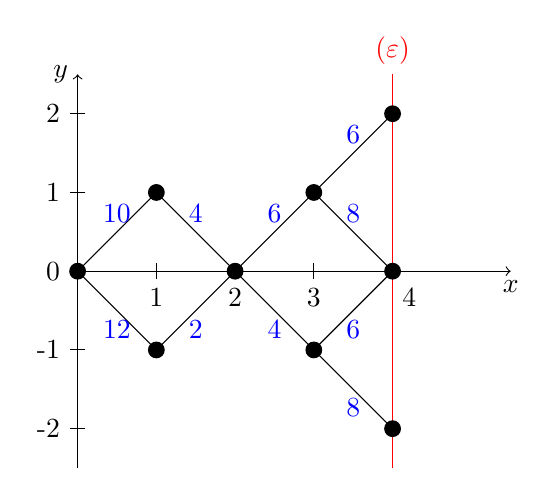
\begin{tikzpicture}
\draw[->] (0,-2.5) -- (0,2.5) node [left] {$y$};
\draw[->] (0,0) -- (5.5,0) node [below] {$x$};
\draw[red] (4,-2.5) -- (4,2.5) node [above] {$(\varepsilon)$};

\draw (0,0) -- (1,-1) node[blue, below, midway] {12};
\draw (1,-1) -- (2,0) node[blue, below, midway] {2};
\draw (2,0) -- (3,-1) node[blue, below, midway] {4};
\draw (3,-1) -- (4,-2) node[blue, below, midway] {8};
\draw (0,0) -- (1,1) node[blue, above, midway] {10};
\draw (1,1) -- (2,0) node[blue, above, midway] {4};
\draw (2,0) -- (3,1) node[blue, above, midway] {6};
\draw (3,1) -- (4,2) node[blue, above, midway] {6};
\draw (3,1) -- (4,0) node[blue, above, midway] {8};
\draw (4,0) -- (3,-1) node[blue, below, midway] {6};

\draw (4,0.1) -- (4,-0.1) node [below right] {4};

\foreach \i in {1,2,3}
    \draw ({\i}, 0.1) -- ({\i},-0.1) node [below] {\i};

\foreach \i in {-2,-1,0,1,2}
    \draw (0.1, {\i}) -- (-0.1, {\i}) node [left] {\i};
    
\node[circle,draw,inner sep=2pt,fill] at (0,0) {};
\node[circle,draw,inner sep=2pt,fill] at (1,1) {};
\node[circle,draw,inner sep=2pt,fill] at (1,-1) {};
\node[circle,draw,inner sep=2pt,fill] at (2,0) {};
\node[circle,draw,inner sep=2pt,fill] at (3,1) {};
\node[circle,draw,inner sep=2pt,fill] at (3,-1) {};
\node[circle,draw,inner sep=2pt,fill] at (4,2) {};
\node[circle,draw,inner sep=2pt,fill] at (4,0) {};
\node[circle,draw,inner sep=2pt,fill] at (4,-2) {};
\end{tikzpicture}
\end{center}

Find the optimal command policy for minimizing the expected cost with the following methods
\begin{enumerate}[label = {\textbf{(\greek*)}}]
    \item optimal control with feedback.
    
    \begin{sol}
    \begin{enumerate}[start = 1, label = {\protect\tsc{$\mathbf{S_{\arabic*}}$}}]
    \item The Optimal Expectation Function (OEF)
    
    $f(x,y):=$ minimum expected cost from $(x,y)$ to $(\varepsilon)$
    
    \item Boundary Condition (BC) at stage $x=3$
    
    $f(3,-3)=f(3,-1)=f(3,1)=f(3,3)=0$
    
    \item Auxiliary functions
    
    \begin{itemize}
        \item $u(x,y)=$ the cost of going from node $(x,y)$ to the upper node $(x+1,y+1)$
        
        \item $l(x,y)=$ the cost of going from node $(x,y)$ to the lower node $(x+1,y-1)$
        
        \item $U(x,y)=$ the minimum expected cost from $(x,y)$ to $(\varepsilon)$ when the command is $u(x,y)$ or use upper path.
        
        \item $L(x,y)=$ the minimum expected cost from $(x,y)$ to $(\varepsilon)$ when the command is $l(x,y)$ or use lower path.
    \end{itemize}
    
    Focus on $U(x,y)$
    
    Command: up 
    $\begin{cases} 
    \text{executed:} & p\rbr{u(x,y)+f(x+1,y+1)} \\
    \text{not executed:} & \rbr{1-p}\rbr{l(x,y)+f(x+1,y-1)} 
    \end{cases}$
    
    $U(x,y)=p(u+f(x+1,y+1)) + (1-p)(l+f(x+1,y-1))$
    
    Focus on $L(x,y)$
    
    $L(x,y)=p(l+f(x+1,y-1)) + (1-p)(u+f(x+1,y+1))$
    
    \item Recursive formula for OEF, using optimization principle.
    
    $$f(x,y)=\min\cbr{U(x,y),L(x,y)}$$
    
    \item \underline{Stage $x=3$}
    
    Nodes $(3,1)$, $(3,-1)$
     \begin{itemize}
        \item Node $(3,1)$
        
        $\begin{aligned}
            U(3,1) &= p(u(3,1)+f(4,2)) + (1-p)(l(3,1)+f(4,0)) \\
            &= 0.6\cdot6 +0.4\cdot8 \\
            &= 6.8
        \end{aligned}$
        
        $\begin{aligned}
            L(3,1) &= p(l(3,1)+f(4,0)) + (1-p)(u(3,1)+f(4,2)) \\
            &= 0.6\cdot8 +0.4\cdot6 \\
            &= 7.2
        \end{aligned}$
        
        \imp $f(3,1)=\min\cbr{6.8,7.2}=6.8$
        
        Command: \textit{up}
        
        \item Node $(3,-1)$
        
        Since $u(3,-1)=u(3,1)$ and $l(3,-1)=l(3,1)$ we get the same $U(x,y)$ and $L(x,y)$, hence 
        
        $f(3,-1)=\min\cbr{6.8,7.2}=6.8$
        
        Command: \textit{up}
    \end{itemize}
    
    \underline{Stage $x=2$}
    \begin{itemize}
    \item Node $(2,0)$
    
    $\begin{aligned}
            U(2,0) &= p(u(2,0)+f(3,1)) + (1-p)(l(2,0)+f(3,-1)) \\
            &= 0.6\rbr{6+6.8} + 0.4\rbr{4+6.8} \\
            &= 0.6\cdot12.8 +0.4\cdot10.8 \\
            &= 12
        \end{aligned}$
        
        $\begin{aligned}
            L(2,0) &= p(l(2,0)+f(3,-1)) + (1-p)(u(2,0)+f(3,1)) \\
            &= 0.6\rbr{4+6.8} + 0.4\rbr{6+6.8} \\
            %&= 0.6\cdot10.8 +0.4\cdot12.8 \\
            &= 11.6
        \end{aligned}$
        
        \imp $f(2,0)=\min\cbr{12,11.6}=11.6$
        
        Command: \textit{down}
    \end{itemize}
    
    \underline{Stage $x=1$}
    Nodes $(1,1)$, $(1,-1)$
    
    Since at each of these nodes, we have only one choice of path, we assume we cannot go wrong with our command (cannot go \textit{off-path}).
    
    \begin{itemize}
        \item Node $(1,1)$
        $f(1,1)=4+f(2,0)=4+11.6=15.6$
        
        Command: \textit{down}
        
        \item Node $(1,-1)$
        $f(1,-1)=2+f(2,0)=2+11.6=13.6$
        
        Command: \textit{up}
    \end{itemize}
    
    \underline{Stage $x=0$}
   \begin{itemize}
       \item Node $O(0,0)$
    
    $\begin{aligned}
            U(0,0) &= p(u(0,0)+f(1,1)) + (1-p)(l(0,0)+f(1,-1)) \\
            &= 0.6\rbr{10+15.6} + 0.4\rbr{12+13.6} \\
            &= 25.6
        \end{aligned}$
        
        $\begin{aligned}
            U(0,0) &= p(l(0,0)+f(1,-1)) + (1-p)(u(0,0)+f(1,1)) \\
            &= 0.6\rbr{12+13.6} + 0.4\rbr{10+15.6} \\
            &= 25.6
        \end{aligned}$
        
        \imp $f(0,0)=\min\cbr{25.6,25.6}=25.6$
        
        Command: \textit{any}
   \end{itemize}
   
   \item Optimal Command Policy
    \begin{itemize}
        \item[$(0,0)$] any
        \item[$(1,1)$] down
        \item[$(1,-1)$] up
        \item[$(2,0)$] down
        \item[$(3,1)$] up
        \item[$(3,-1)$] up
    \end{itemize}
    
    \end{enumerate}
    \end{sol}
    \item open cycle, where paths containing the same direction three times in row (UUU or LLL) are not possible and therefore not commanded.
    
    \begin{sol}
    \begin{enumerate}[start = 1, label = {\protect\tsc{$\mathbf{S_{\arabic*}}$}}]
\item Possible command sequences:

$\begin{array}{cccc}
    \text{ULUU} & \text{ULUL} & \text{ULLU} & \text{ULLL}  \\
    \text{LUUU} & \text{LUUL} & \text{LULU} & \text{LULL}  
\end{array}$

But we cannot give commands $\text{ULLL}$ or $\text{LUUU}$ since we cannot give the same command 3 times in a row.

So we have commands 

$\begin{array}{cccc}
    \text{ULUU} & \text{ULUL} & \text{ULLU} &   \\
         & \text{LUUL} & \text{LULU} & \text{LULL}  
\end{array}$

We study each seperately.

We assume that if a command is taken, which was not executed (opposite direction taken) and hence the same direction is taken 3 times in a row (e.g. command given is $\text{ULLU}$ but the final direction is not executed, so the actual path taken is $\text{ULLL}$) then this is possible.

We also assume the first two commands $UL$ or $LU$ are taken together, since there is only one choice of path at $x=1$ (as discussed in the previous part).

\item Focus on $\text{ULUU}$ (commands: up, down, up, up)

\begin{tabular}{llcl}
    Path & Cost & \quad & Probability  \\
    $\text{ULUU}$ & $10+4+6+6=26$ & & $p^3$ \\
    $\text{ULUL}$ & $10+4+6+8=28$ & & $p^2(1-p)$ \\
    $\text{ULLU}$ & $10+4+4+6=24$ & & $p^2(1-p)$ \\
    $\text{ULLL}$ & $10+4+4+8=26$ & & $p(1-p)^2$ \\
    $\text{LUUU}$ & $12+2+6+6=26$ & & $p^2(1-p)$ \\
    $\text{LUUL}$ & $12+2+6+8=28$ & & $p(1-p)^2$ \\
    $\text{LULU}$ & $12+2+4+6=24$ & & $p(1-p)^2$ \\
    $\text{LULL}$ & $12+2+4+8=26$ & & $(1-p)^3$ 
\end{tabular}

Then 

$\begin{aligned}
    \bE(\text{ULUU}) &= \sum (\text{Cost})(\text{probability}) \\
    &= 26\times 0.6^3 + 28\times 0.6^2\times 0.4 + 24\times 0.6^2\times 0.4 + 26\times 0.6\times0.4^2 \\
    &+ 26\times 0.6^2\times 0.4 + 28\times 0.6\times 0.4^2 + 24\times 0.6\times 0.4^2 + 26\times 0.4^3 \\
    &= 26
\end{aligned}$


Focus on $\text{ULUL}$ (commands: up, down, up, down)

Similarly we can work out the cost of taking each path and their corresponding probabilities

$\begin{aligned}
    \bE(\text{ULUL}) &= 28\times 0.6^3 + 26\times 0.6^2\times 0.4 + 26\times 0.6^2\times 0.4 + 24\times 0.6\times0.4^2 \\
    &+ 28\times 0.6^2\times 0.4 + 26\times 0.6\times 0.4^2 + 26\times 0.6\times 0.4^2 + 24\times 0.4^3 \\
    &= 26.4
\end{aligned}$

Focus on $\text{ULLU}$ (commands: up, down, down, up)

$\begin{aligned}
    \bE(\text{ULLU}) &= 24\times 0.6^3 + 26\times 0.6^2\times 0.4 + 26\times 0.6^2\times 0.4 + 24\times 0.6\times0.4^2 \\
    &+ 24\times 0.6^2\times 0.4 + 26\times 0.6\times 0.4^2 + 26\times 0.6\times 0.4^2 + 28\times 0.4^3 \\
    &= 25.6
\end{aligned}$

Focus on $\text{LUUL}$ (commands: down, up, up, down)

Notice that this will have the same expected cost as $\text{ULUL}$, since the first two steps $UL$ and $LU$ both have cost $14$.

Therefore $\bE(\text{LUUL})=26.4$

Focus on $\text{LULU}$ (commands: down, up, down, up)

Similarly, this will have the same expected cost as $\text{ULLU}$, since the first two steps $UL$ and $LU$ both have cost $14$.

Therefore $\bE(\text{LULU})=25.6$

Focus on $\text{LULL}$ (commands: down, up, down, down)

$\begin{aligned}
    \bE(\text{LULL}) &= 26\times 0.6^3 + 24\times 0.6^2\times 0.4 + 28\times 0.6^2\times 0.4 + 26\times 0.6\times0.4^2 \\
    &+ 26\times 0.6^2\times 0.4 + 24\times 0.6\times 0.4^2 + 28\times 0.6\times 0.4^2 + 24\times 0.4^3 \\
    &= 26
\end{aligned}$

\item Minimum expected cost

$\min\cbr{\bE(\text{ULUU}),\bE(\text{ULUL}),\bE(\text{ULLU}),\bE(\text{LUUL}),\bE(\text{LULU}),\bE(\text{LULL})}=25.6$

Optimal command sequence: $\text{ULLU}$ or $\text{LULU}$

\end{enumerate}
    \end{sol}
\end{enumerate}
\end{prob}